\section{Protocolo IP}

La \textbf{capa de enlace} (capa 2) se encarga de proveer conectividad entre nodos adyacentes o vecinos, siendo responsable de transmitir una trama sobre un enlace en particular. Los mensajes entre origen y destino pueden transitar por distintas capas de enlace. La \textbf{Capa de Red} se encuentra por encima de la capa de enlace.

\begin{figure}[htbp]
    \centering
    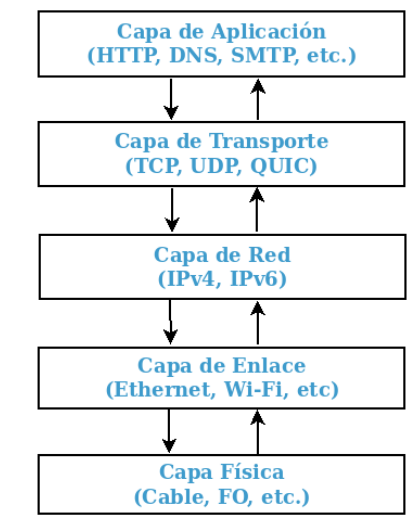
\includegraphics[width=0.5\textwidth]{capitulos/ip/imagenes/capas.png}
    \caption{Modelo TCP/IP}
    \label{fig:capas-de-modelo-tcp}
\end{figure}

\subsection{Diseño y Servicios}

La capa de red fué diseñada para que cumpla con los siguientes requerimientos: 

\noindent
\begin{enumerate}[label=\textcolor{acento}{$\bullet$}]
    \item Independiente de la tecnología de subred.
    \item Aislada de la cantidad, tipo y topologías de las \textbf{subredes}.
    \item Direccionamiento uniforme.
\end{enumerate}

Como servicios, debe poder transportar mensajes desde un nodo emisor a receptor (inclusive si son redes distintas) y determinar el camino que seguirá un mensaje entre dos nodos. Al no ser orientado a conexión, no brinda ni control de errores, ni secuenciamiento ni confiabilidad: es un servicio de \textbf{Best-Effort}.

\begin{definicion}{Protocolo Best-Effort}
    Hay independencia en cuanto al envío a través de la red, haciendo posible que los paquetes puedan llegar desordenados o seguir caminos diferentes. Tampoco hay control de errores. 
\end{definicion}

Tiene dos funcionalidades principales:

\begin{itemize}[label=\textcolor{acento}{$\bullet$}]
    \item Direccionamiento
    \item Ruteo
\end{itemize}

También se encarga de multiplexar o demultiplexar protocolos superiores, y puede fragmentar paquetes.

\begin{figure}[htbp]
    \centering
    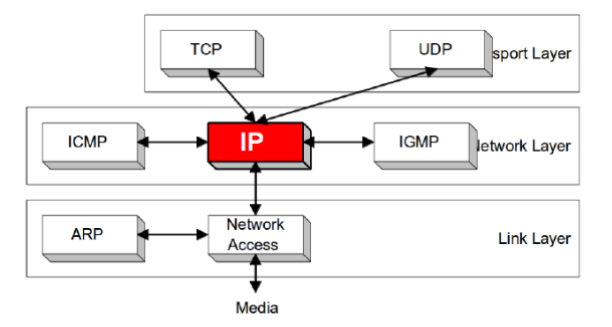
\includegraphics[width=0.5\textwidth]{capitulos/ip/imagenes/capas-relativo-ip.png}
    \caption{Modelo TCP/IP}
    \label{fig:capas-relativo-ip}
\end{figure}

\subsection{Estructura del Datagrama IP}

El \textbf{Datagrama IP} tiene longitud variable. Está compuesto por dos partes: header y payload. El \textbf{Header} tiene una longitud de entre 20 y 60 bytes.

\begin{figure}[htbp]
    \centering
    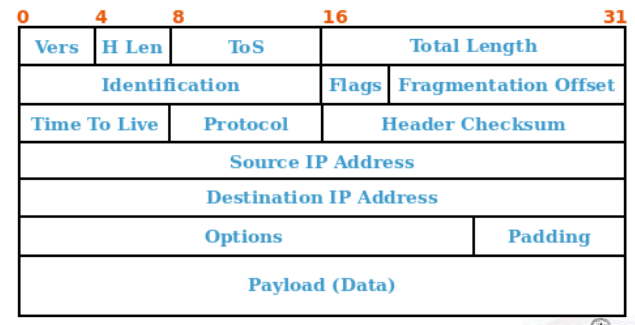
\includegraphics[width=0.5\textwidth]{capitulos/ip/imagenes/ip-datagram.png}
    \caption{Datagrama IP}
    \label{fig:ip-datagram}
\end{figure}

Los campos más relevantes son: 

\begin{itemize}[label=\textcolor{acento}{$\bullet$}]
    \item \textbf{Header Lenght:} longitud del header, en palabras de 32 bits.
    \item \textbf{Type of Service (TOS):} confiabilidad, prioridad, retardo y throughput.
    \item \textbf{Identification:} número único para segmentos del mismo datagrama.
    \item \textbf{Flags:} 
    \begin{itemize}[label=\textcolor{primario!60}{$\bullet$}]
        \item X = reservado. 
        \item D = Don't Fragment. Si es 0 puede fragmentarse, si es 1 no.
        \item M = More Fragments. Si es 0 es el último fragmento, si es 1 no.
    \end{itemize}
    \item \textbf{Fragment Offfset:} el desplazamiento del segmento dentro del datagrama original. Está dado en múltiplos de 8 bytes.
    \item \textbf{Time To Live (TTL):} número que se decrementa cada vez que llega a un router, y cuando llega a 0 se descarta. Es utilizado para evitar loops.
    \item \textbf{Protocol:} protocolo contenido en el campo de datos (UDP, TCP, ICMP, ...).
\end{itemize}

\subsection{Direccionamiento IP}

Las direcciones IP identifican unívocamente una intefraz de red. Los routers pueden tener más de una dirección IP, y a diferencia de las direcciones MAC, estas direcciones son lógicas.

Hay distintos tipos de direcciones: 

\begin{itemize}[label=\textcolor{acento}{$\bullet$}]
    \item \textbf{Unicast:} destinada a un host/interface en particular.
    \item \textbf{Broadcast:} destinada a todos los hosts de una red.
    \item \textbf{Multicast:} destinada a un grupo de hosts de una o varias redes.
\end{itemize}

Además de estas direcciones, también está la de \emph{Loopback} (127.0.0.1) y la utilizada cuando aún no se le asignó una red al dispositivo (0.0.0.0).

\subsubsection{Subnetting}

El subnetting es el proceso de dividir una red física o lógica de gran tamaño en subredes más pequeñas. Esto se logra alterando la máscara de red predeterminada, ``pidiendo prestados'' bits de la porción destinada a los hosts para asignarlos a la porción de red.


\begin{itemize}[label=\textcolor{acento}{$\bullet$}]
    \item \textbf{Objetivo:} Reducir el tamaño de los dominios de broadcast, mejorar la seguridad, facilitar la administración y evitar el desperdicio de direcciones IP dentro de una organización.
    \item \textbf{Mecanismo:} Se desplaza el límite de la máscara de red hacia la derecha (aumenta el prefijo).
    \item \textbf{Cálculo de Subredes y Hosts:} 
    Si se toman $n$ bits prestados de la porción de host, se pueden crear $2^n$ subredes. En cada subred, si quedan $h$ bits para los hosts, habrá $2^h - 2$ direcciones utilizables (se restan 2 por las direcciones de red y de broadcast).
\end{itemize}

\subsection{VLSM (Variable Length Subnet Mask)}
El subnetting tradicional (FLSM) divide una red en subredes del mismo tamaño, lo que a menudo sigue generando desperdicio. \textbf{VLSM} mejora esto permitiendo aplicar diferentes máscaras de subred dentro del mismo bloque de direcciones mayor. Al hacer subnetting de una subred previamente dividida, los bloques se ajustan estrictamente a la cantidad de hosts necesarios para cada departamento o enlace.

\begin{nota}{\textbf{Ejemplo de Subnetting} \newline}
    Dada la red $192.168.10.0/24$, si necesitamos una red para 80 hosts (requiere 7 bits, $2^7-2 = 126$), utilizamos un prefijo $/25$. La dirección sería $192.168.10.0/25$. El segmento sobrante, $192.168.10.128/25$, se puede seguir dividiendo con prefijos mayores (como $/26$, $/27$) para áreas que requieran menos hosts.    
\end{nota}

\subsubsection{Supernetting (Sumarización)}

El supernetting o \textbf{CIDR (Classless Inter-Domain Routing)}, es el proceso conceptualmente opuesto al subnetting. Consiste en combinar o agrupar múltiples redes contiguas más pequeñas en una única red o ruta más grande.

\begin{itemize}[label=\textcolor{acento}{$\bullet$}]
    \item \textbf{Objetivo:} Reducir drásticamente el tamaño de las tablas de ruteo en los routers de núcleo (core routers) de Internet y optimizar el procesamiento de rutas.
    \item \textbf{Mecanismo:} Se desplaza el límite de la máscara de red hacia la izquierda (disminuye el tamaño del prefijo), agrupando los bits de red compartidos.
    \item \textbf{Requisitos para la Sumarización:} Para agrupar redes, estas deben ser contiguas, el número de redes a agrupar debe ser potencia de 2, y las redes deben compartir exactamente los mismos bits de red de orden superior.
\end{itemize}


Ahora un \textbf{ejemplo}. Supongamos que un router tiene en su tabla las siguientes cuatro rutas hacia subredes contiguas:
\begin{itemize}
    \item $192.168.0.0/24$ (En binario el tercer octeto es: $00000000$)
    \item $192.168.1.0/24$ (En binario el tercer octeto es: $00000001$)
    \item $192.168.2.0/24$ (En binario el tercer octeto es: $00000010$)
    \item $192.168.3.0/24$ (En binario el tercer octeto es: $00000011$)
\end{itemize}

Dado que las cuatro redes comparten los primeros 22 bits ($192.168.000000XX$), se pueden agrupar en una única entrada en la tabla de enrutamiento reduciendo la máscara a $/22$. La ruta resumida resultante será:
$$\mathbf{192.168.0.0/22}$$

\subsubsection{Cuadro Comparativo}
\small
\setlength{\tabcolsep}{4pt}
{\renewcommand{\arraystretch}{1.5}
\begin{table}[h!]
\centering
\begin{tabular}{@{} >{\RaggedRight\arraybackslash}p{3.8cm} >{\RaggedRight\arraybackslash}p{5.3cm} >{\RaggedRight\arraybackslash}p{5.3cm} @{}}
\toprule
\textbf{Característica} & \textbf{Subnetting} & \textbf{Supernetting (CIDR)} \\
\midrule
\textbf{Definición} & Divide una red en redes más pequeñas. & Agrupa redes pequeñas en una más grande. \\
\textbf{Movimiento de Máscara} & Hacia la derecha (aumenta el prefijo, ej. $/24 \rightarrow /26$). & Hacia la izquierda (reduce el prefijo, ej. $/24 \rightarrow /22$). \\
\textbf{Problema que Resuelve} & Agotamiento interno de IPs y dominios de broadcast grandes. & Crecimiento desmedido de las tablas de ruteo globales. \\
\textbf{Bits alterados} & Toma bits de \textit{Host} para hacer \textit{Red}. & Toma bits de \textit{Red} para hacer \textit{Host}. \\
\bottomrule
\end{tabular}
\end{table}
}

\subsection{Routing}

Acción donde se selecciona el próximo salto de un paquete, y su interfaz de salida. Los routers y hosts pueden hacer routing. Es una acción de control, cuyo motor son los protocolos de enrutamiento. Las tablas de ruteo estan compuestas por:

\begin{itemize}[label=\textcolor{acento}{$\bullet$}]
    \item Red Destino
    \item Máscara de Red (o Prefijo)
    \item Next Hop (Próximo Salto)
    \item Interface de Salida
    \item Métrica
\end{itemize}

\begin{nota}{\textbf{Recordar} \newline}
    Solo puede haber un default gateway por tabla de ruteo.
\end{nota}

A diferencia del routing, el \textbf{Forwarding} consiste en pasar un mensaje desde una interfaz de entrada hacia una de salida, por donde envía los mensajes de los protocolos enrutados. 

\subsection{Fragmentación}

\begin{definicion}{Maximum Transfer Unit (MTU)}
    Es el tamaño máximo de paquete permitido en un enlace. 
\end{definicion}

Un datagrama puede pasar por varias capas de enlaces con distintos MTUs, y los datagramas con tamaño mayor al MTU deben ser fragmentados con tamaño \textbf{múltiplo de 8 bytes} (excepto el último). Cada fragmento pasa a ser un nuevo paquete, donde el header se copia del original y luego se modifican los campos necesarios. 

El \textbf{Path MTU} permite saber el mínimo MTU entre origen y destino.


\begin{figure}[htbp]
    \centering
    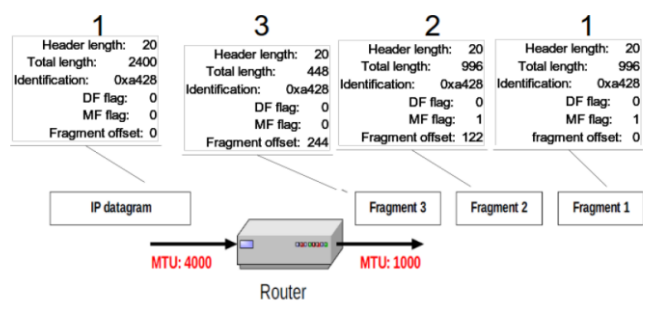
\includegraphics[width=0.5\textwidth]{capitulos/ip/imagenes/fragmentacion.png}
    \caption{Fragmentación en IP}
    \label{fig:fragmentacion-ip}
\end{figure}

Los datagramas se reconstruyen en el destino final una vez que llegan todos los fragmentos, que pueden tomar distintos caminos. Estos fragmentos pueden a su vez fragmentarse de nuevo. En caso de que no lleguen \textbf{todos} los fragmentos, el paquete entero se descarta.







